% ============================================================
%  WIT-2021-ATIYAH-LANG 幻灯片版（中文译注）
%  编译：xelatex main.tex 两遍
% ============================================================
\documentclass[aspectratio=169,12pt]{ctexbeamer}

\usepackage{amsmath,amssymb,mathtools,bm}
\usepackage{booktabs}
\usepackage{array}
\usepackage{tcolorbox}
\tcbuselibrary{skins}
\usepackage{tikz}
\usetikzlibrary{positioning,arrows.meta,calc,decorations.pathmorphing}

% ---------- 外观：白底、衬线、无导航条，仿 Witten 的幻灯片 ----------
\setbeamertemplate{navigation symbols}{}
\setbeamercolor{normal text}{fg=black!90}
\setbeamercolor{frametitle}{fg=black}
\setbeamercolor{structure}{fg=black!65}
\setbeamerfont{frametitle}{family=\rmfamily,series=\bfseries,size=\Large}
\setbeamerfont{normal text}{size=\large}
\setlength{\parskip}{0.55em}
\setlength{\parindent}{0pt}
\setbeamertemplate{footline}{%
  \hfill{\color{black!45}\scriptsize\insertframenumber\,/\,\inserttotalframenumber}%
  \hspace{1.4em}\vspace{0.85em}}

% ---------- 记号 ----------
\newcommand{\CC}{\mathbb{C}}
\newcommand{\RR}{\mathbb{R}}
\newcommand{\ZZ}{\mathbb{Z}}
\newcommand{\PP}{\mathbb{P}}
\newcommand{\HH}{\mathbb{H}}
\newcommand{\cO}{\mathcal{O}}
\newcommand{\cL}{\mathcal{L}}
\newcommand{\cE}{\mathcal{E}}
\newcommand{\cF}{\mathcal{F}}
\newcommand{\cG}{\mathcal{G}}
\newcommand{\cH}{\mathcal{H}}
\newcommand{\cM}{\mathcal{M}}
\newcommand{\cN}{\mathcal{N}}
\newcommand{\cT}{\mathcal{T}}
\newcommand{\cD}{\mathcal{D}}
\newcommand{\cB}{\mathcal{B}}
\newcommand{\cA}{\mathcal{A}}
\newcommand{\dd}{\mathrm{d}}
\newcommand{\ee}{\mathrm{e}}
\newcommand{\ii}{\mathrm{i}}
\newcommand{\gvee}{G^{\vee}}
\newcommand{\Tvee}{T^{\vee}}
\newcommand{\Hom}{\operatorname{Hom}}
\newcommand{\Tr}{\operatorname{Tr}}
\newcommand{\End}{\operatorname{End}}
\newcommand{\Aut}{\operatorname{Aut}}
\newcommand{\SL}{\mathrm{SL}}
\newcommand{\SU}{\mathrm{SU}}
\newcommand{\SO}{\mathrm{SO}}
\newcommand{\Sp}{\mathrm{Sp}}
\newcommand{\GL}{\mathrm{GL}}
\newcommand{\PSU}{\mathrm{PSU}}
\newcommand{\ad}{\operatorname{ad}}
\newcommand{\Gr}{\mathrm{Gr}}
\newcommand{\Bun}{\mathrm{Bun}}
\newcommand{\Perv}{\mathrm{Perv}}
\newcommand{\Rep}{\mathrm{Rep}}
\newcommand{\srcp}[1]{{\color{black!40}\scriptsize[原 p.#1]}}

% ---------- 两种补注框 ----------
\newtcolorbox{beizhu}{enhanced, colback=blue!3!white, colframe=blue!3!white,
  borderline west={1.1pt}{0pt}{blue!45!black},
  boxrule=0pt, left=7pt, right=5pt, top=3pt, bottom=3pt,
  fontupper=\small, before skip=6pt, after skip=2pt}
\newtcolorbox{yizhu}{enhanced, colback=orange!4!white, colframe=orange!4!white,
  borderline west={1.1pt}{0pt}{orange!70!black},
  boxrule=0pt, left=7pt, right=5pt, top=3pt, bottom=3pt,
  fontupper=\small, before skip=6pt, after skip=2pt}

% ---------- 分部页 ----------
\newcommand{\partframe}[2]{%
\begin{frame}[plain]
  \vspace*{2.6cm}
  {\color{black!35}\large 第 #1 部分}\\[0.8em]
  {\LARGE\bfseries #2}\\[1.2em]
  {\color{black!40}\rule{2.2cm}{0.4pt}}
\end{frame}}

\title{对偶、Langlands 对应\\ 与 Michael Atiyah 的影响}
\author{Edward Witten\quad（2021 年 9 月 23 日，Isaac Newton Institute）}
\date{中文译注本 · 2026}

\begin{document}

% ===================== 封面 =====================
\begin{frame}[plain]
\vspace*{1.1cm}
{\color{black!45}\small 数译 · 威腾演讲译注}\\[1.2em]
{\LARGE\bfseries 对偶、Langlands 对应\\[0.45em] 与 Michael Atiyah 的影响}\\[1.3em]
{\large Edward Witten}\\[0.5em]
{\normalsize 2021 年 9 月 23 日 · 剑桥 Isaac Newton Institute}\\[1.5em]
{\color{black!40}\rule{2.6cm}{0.4pt}}\\[1.2em]
{\small 中文译注本 · 幻灯片版}\quad{\color{black!50}\small 超对称梦想家　译注}
\end{frame}

% ===================== 路线图 =====================
\begin{frame}{这场演讲在讲什么}
  Atiyah 在 1977 年说过一句话：\emph{GNO 所谓的“磁规范群”，就是数论里的
  Langlands 对偶群。}这句话把两条看似无关的线索接在一起。
  \begin{center}
  \begin{tikzpicture}[x=1cm,y=1cm,>={Stealth[length=2mm]},every node/.style={font=\footnotesize}]
    \node[align=left,text width=4.1cm,anchor=north west] (a) at (0,0)
      {\textbf{电磁对偶}\\ GNO $1977$\\ Montonen--Olive $1977$\\ Witten--Olive $1978$};
    \node[align=left,text width=4.3cm,anchor=north west] (b) at (4.6,0)
      {\textbf{超对称与单极子}\\ Osborn $1979$\\ Bogomolny 方程\\ Atiyah--Hitchin $1988$};
    \node[align=left,text width=4.3cm,anchor=north west] (c) at (9.4,0)
      {\textbf{几何 Langlands}\\ Beilinson--Drinfeld $1990$\\ Hecke 特征层\\ Kapustin--Witten $2006$};
    \draw[->] (a.east) -- (b.west);
    \draw[->] (b.east) -- (c.west);
    \draw[->,rounded corners] (a.south) ++(0.9,0) -- ++(0,-0.75) -| node[pos=0.25,below]{Sen $1994$ · Seiberg--Witten $1994$} ++(9.4,-0.75);
  \end{tikzpicture}
  \end{center}
  \begin{beizhu}
  \textbf{批注}\quad 这场演讲不是综述，而是一条“谁在何时想到了什么”的证词：它第一次把 1977 年
  那句口头提醒的后果讲全——从磁荷的群论，到四维流形的微分拓扑。
  \end{beizhu}
\end{frame}

\begin{frame}{读法：三种入口}
  \begin{itemize}
    \item \textbf{想看物理}：第 2--5 部分。电磁对偶的群论、BPS 界、Seiberg--Witten 解。
    \item \textbf{想看数学}：第 6--8 部分。Hecke 修改、几何 Satake、't Hooft 算子与 Hecke 函子。
    \item \textbf{想看“物理为什么能算 Langlands”}：第 9 部分。4d $\cN=4$ 的扭化、二维 sigma 模型、镜像对称。
  \end{itemize}
  \vspace{0.5em}
  记号：$G$ 单连通单群，$T\subset G$ 极大环面，$\gvee$ 为 Langlands 对偶群；
  $X^*(T)=\Hom(T,U(1))$ 特征标格，$X_*(T)=\Hom(U(1),T)$ 余特征标格。
  \[
    \boxed{\;X^*(\Tvee)=X_*(T),\qquad X_*(\Tvee)=X^*(T)\;}
  \]
\end{frame}

\partframe{一}{1977：一句口头提醒}

% ===================== Part I =====================
\begin{frame}{哈佛，1977 年春}
  \srcp{2} 那年春天我在哈佛做 Junior Fellow。Michael Atiyah 来哈佛讲学，讲的是瞬子。
  我听完很受触动，去和他交谈；他邀我在当年年底访问牛津。
  \vspace{0.4em}

  那年年底我到了牛津。整个访问期间，Michael 讲的是四维规范理论里的瞬子。他和
  Vladimir Drinfeld、Nigel Hitchin、Yuri Manin 刚刚借助扭量理论与代数几何发现了
  瞬子的 ADHM 构造。
  \begin{beizhu}
  \textbf{批注（ADHM）}\quad $\RR^4$ 上 $SU(N)$ 瞬子（自对偶联络，拓扑荷 $k$）的模空间
  等同于线性数据
  \[
    (B_1,B_2,I,J)\in\End(\CC^k)^{\oplus2}\oplus\Hom(\CC^N,\CC^k)\oplus\Hom(\CC^k,\CC^N)
  \]
  在实矩映射方程 $[B_1,B_1^\dagger]+[B_2,B_2^\dagger]+II^\dagger-J^\dagger J=0$、
  $[B_1,B_2]+IJ=0$ 的零点集上模去 $U(k)$。非线性椭圆方程，被写成了有限维线性代数。
  \end{beizhu}
\end{frame}

\begin{frame}{为什么瞬子那么重要}
  \srcp{2} 瞬子当时是物理里最令人兴奋的题目之一，很大程度上是因为 Gerard 't Hooft 的工作：
  他用瞬子解决了核力的“$U(1)$ 问题”。
  \vspace{0.4em}

  到 1977 年底，我们又从 Albert Schwarz 的一个观察知道，'t Hooft 关于 $U(1)$ 问题的工作
  可以理解为 Atiyah--Singer 指标定理的一次应用。
  \begin{beizhu}
  \textbf{批注（$U(1)$ 问题）}\quad 按照手征对称性，九种赝标介子中应当有一个很轻的粒子，
  但实验上 $\eta'$ 的质量却大得多。't Hooft 指出：瞬子通过费米子的零模诱导出一个破坏
  $U(1)$ 的有效相互作用；而零模的个数恰由 Dirac 算子的指标给出，也就是由瞬子的拓扑荷给出。
  这正是“物理的量子数 $=$ 几何的指标”的第一次显式兑现。
  \end{beizhu}
\end{frame}

\begin{frame}{Atiyah 换了题目}
  \srcp{3} 那个月的大部分时间，我们都在热烈地讨论瞬子。但到了月底，Atiyah 换了题目。
  他让我注意两篇我没见过的物理论文：
  \begin{itemize}
    \item Peter Goddard、Jean Nuyts 与 David Olive，\emph{Gauge Theories and Magnetic Charge}
      （Nuclear Physics B125, 1977）；
    \item David Olive 与 Claus Montonen，\emph{Magnetic Monopoles as Gauge Particles?}
      （Physics Letters B72, 1977）。
  \end{itemize}
  他说他觉得这里面有很深的东西，我应该去伦敦和 Olive 谈谈。
\end{frame}

\begin{frame}{两篇文章的共同点：把“磁”看成“另一套群”}
  \begin{columns}[T]
  \begin{column}{0.49\textwidth}
    \textbf{GNO}：磁荷的算子是 $H$ 的生成元的线性组合，其分量在 Weyl 群下唯一确定，
    并且必须是某个新群 $H^0$ 的权。$H$ 与 $H^0$ 互为“电/磁”，$(H^0)^0=H$。
  \end{column}
  \begin{column}{0.49\textwidth}
    \textbf{Montonen--Olive}：量子化之后，'t Hooft--Polyakov 单极子与光子组成同一个规范
    多重态；对应的拉氏量与原 Georgi--Glashow 模型相同，只是把电电荷换成了磁电荷。
  \end{column}
  \end{columns}
  \vspace{0.5em}
  \begin{beizhu}
  \textbf{批注}\quad 两篇文章的年代相同（1977），但气质不同：GNO 是群论与拓扑的静态陈述，
  MO 是量子动力学的猜想。把它们连起来的，正是 Atiyah 的那句提醒。
  \end{beizhu}
\end{frame}

\begin{frame}{Atiyah 的那句话}
  \srcp{6} Atiyah 向我解释：Goddard、Nuyts 与 Olive 所谓的“磁规范群”，
  其实就是数论 Langlands 纲领里的 Langlands 对偶群。
  \vspace{0.4em}

  我相当确定这个联系是 Atiyah 做出的，但据我所知他从未把它写下来。和当时别的物理学家
  一样，我从未听过 Langlands 纲领，也没听过 Robert Langlands 这个名字。但 Atiyah 向我
  保证：数论的 Langlands 纲领是非常深刻的东西，他认为物理学家必定也在通向某种重要的东西。
  \begin{beizhu}
  \textbf{批注}\quad 这条口头传统在物理文献里第一次被明确引用，要等到 2006 年
  Kapustin 与 Witten 的论文。本书的整个叙事，可以看作对这句话的展开与验证。
  \end{beizhu}
\end{frame}

\partframe{二}{电荷、磁荷与对偶群}

\begin{frame}{$U(1)$：电电荷就是表示}
  \srcp{7} 先看阿贝尔情形 $G=U(1)$，即现实世界里的电磁规范群。所谓“带电粒子”，
  最根本的定义是：粒子对应 $G$ 的一个表示。
  \vspace{0.4em}

  因为 $U(1)$ 的每个表示都是基本表示的 $n$ 次幂，电电荷就可以看成一个整数 $n$。
  换一种不抽象的说法：电荷是“量子化”的，任何粒子的电荷都是电子电荷的整数倍。
  \[
    \text{电电荷}\;\longleftrightarrow\;\text{表示}\;\longleftrightarrow\; n\in\ZZ
    \;\longleftrightarrow\; X^*(U(1))\cong\ZZ .
  \]
\end{frame}

\begin{frame}{Dirac 单极子：奇点与第一陈类}
  \srcp{8} 在 $U(1)$ 规范理论里，“规范场”是某个复线丛 $\cL$ 上的联络 $A$，曲率 $F=\dd A$。
  电子的量子波函数是 $\cL$ 的截面 $\psi$。

  Dirac 的单极子概念是：单极子的位置是空间中的一个奇点 $p$，在那里线丛 $\cL$ 与联络 $A$
  没有定义；$\RR^3\setminus\{p\}$ 中围绕 $p$ 的二维球面 $S$ 可缩，磁荷是
  \[
    m=\int_S c_1(\cL)\in\ZZ .
  \]
  \begin{center}
  \begin{tikzpicture}[scale=0.62,>={Stealth[length=1.6mm]}]
    \shade[ball color=black!12] (0,0) circle (1.5);
    \draw[black!45,dashed] (-1.5,0) arc (180:360:1.5 and 0.45);
    \draw[black!45] (-1.5,0) arc (180:0:1.5 and 0.45);
    \fill (0.35,0.55) circle (1.6pt) node[right,font=\scriptsize]{$p$};
    \node at (-1.9,1.55) {\scriptsize $S$};
    \node[font=\scriptsize,black!60] at (2.5,0.55) {$\cL,A$ 在 $p$ 处无定义};
  \end{tikzpicture}
  \end{center}
\end{frame}

\begin{frame}{Dirac 量子化：$e\int_S F\in2\pi\ZZ$}
  设 $F$ 是 $S$ 上的曲率，$e$ 是试探电荷。沿闭合路径的相位是 $\exp(\ii e\oint A)$；
  若把 $S$ 分成两个半球 $D_\pm$，在赤道上 $A_+-A_-=\dd\log g$，$g:S^1\to U(1)$。
  波函数的单值性要求
  \[
    \exp\!\Big(\ii e\oint_{S^1}A_+-A_-\Big)=1
    \quad\Longleftrightarrow\quad
    e\int_S F\in 2\pi\ZZ .
  \]
  而 $\int_S F=2\pi m$，所以
  \[
    e\,m\in 2\pi\ZZ\cdot\frac{1}{2\pi}\;\Longrightarrow\; em\in 2\pi\ZZ .
  \]
  \begin{beizhu}
  \textbf{批注}\quad 这里 $m$ 的归一化使 $\int_S F=2\pi m$（即 $F/2\pi$ 的 de Rham 类给出
  $c_1$）。等价地，磁荷 $g$（使通量 $=4\pi g$）满足 $eg\in2\pi\ZZ$，即 $g=m/2$。
  真正的不变量是配对 $X^*(T)\otimes X_*(T)\to\ZZ$，而不是某个具体数字。
  \end{beizhu}
\end{frame}

\begin{frame}{非阿贝尔：电是表示，磁是拓扑}
  \srcp{10} 现在设 $G$ 是单的非阿贝尔群。时空上有 $G$-丛 $E$，带联络 $A$，曲率
  $F=\dd A+A\wedge A$。
  \begin{itemize}
    \item \textbf{电电荷}容易：任何粒子的电电荷都是 $G$ 的一个表示 $R$。
    \item \textbf{磁荷}微妙：单极子是空间中的一点（或一小块区域），在那里 $E$ 与 $A$ 没有定义；
      磁荷分类的是围绕该点的二维球面 $S$ 上 $G$-丛的选择。
  \end{itemize}
  按这个解释，磁荷取值于 $\pi_1(G)$。
  \begin{beizhu}
  \textbf{批注}\quad $S^2=D^2_+\cup D^2_-$，两个圆盘上的丛都平凡，粘合数据是
  $S^1\to G$ 的映射，其同伦类正是 $\pi_1(G)$。但对单连通的 $G$（如 $SU(2)$），
  $\pi_1(G)=0$：光滑的单极子根本不存在。这就是 GNO 不满意的地方。
  \end{beizhu}
\end{frame}

\begin{frame}{GNO 的出路：希格斯化到极大环面}
  \srcp{11} GNO 考虑的是一种理论：通过希格斯机制，规范群在低能下被有效约化到极大环面
  $T\subset G$。这种约化只在远离 $p$ 的地方发生。
  \vspace{0.4em}

  于是我们可以定义分类 $S$ 上 $T$-丛（而不是 $G$-丛）的磁荷，它取值于
  \[
    \pi_1(T)\;\cong\;\Hom(U(1),T)=X_*(T).
  \]
  另一方面，一旦规范对称性被约化到 $T$，电电荷就应当用 $T$ 的表示来分类；
  而 $T$ 阿贝尔，不可约表示都是一维的：
  \[
    \text{电电荷}\in\Hom(T,U(1))=X^*(T).
  \]
  \begin{beizhu}
  \textbf{批注}\quad 关键的一步：磁荷的“群”从 $\pi_1(G)$ 换成了 $\pi_1(T)=X_*(T)$。
  这一步把拓扑问题变成了格的问题，也才让对偶成为可能。
  \end{beizhu}
\end{frame}

\begin{frame}{两个格}
  \begin{center}
  \renewcommand{\arraystretch}{1.25}
  \begin{tabular}{@{}lll@{}}
    \toprule
    情形 & 电电荷 & 磁荷 \\
    \midrule
    $G=U(1)$ & $n\in\ZZ$ & $m=\int_S c_1(\cL)\in\ZZ$ \\
    非阿贝尔 $G$ & $G$ 的表示 $R$ & 朴素看法：$\pi_1(G)$ \\
    $G$ 破缺到 $T$ & $\Hom(T,U(1))=X^*(T)$ & $\Hom(U(1),T)=X_*(T)$ \\
    \bottomrule
  \end{tabular}
  \end{center}
  \vspace{0.6em}
  注意两个格之间有一个自然的整值配对：
  \[
    \langle \chi,\lambda\rangle=\chi\circ\lambda\in\Hom(U(1),U(1))=\ZZ,
    \qquad \chi\in X^*(T),\;\lambda\in X_*(T).
  \]
  这个配对就是电荷量子化与 Dirac 量子化的群论内容。
\end{frame}

\begin{frame}{GNO 对偶 $=$ 根数据对偶}
  \srcp{13} GNO 观察到：对任何单群 $G$，存在另一个单群 $\gvee$ 与极大环面 $\Tvee$，使得
  \[
    \Hom(T,U(1))=\Hom(U(1),\Tvee),\qquad
    \Hom(U(1),T)=\Hom(\Tvee,U(1)).
  \]
  用格写就是
  \[
    X^*(T)=X_*(\Tvee),\qquad X_*(T)=X^*(\Tvee).
  \]
  \begin{beizhu}
  \textbf{批注（根数据）}\quad $G$ 的根数据是四元组 $(X^*(T),\Phi,X_*(T),\Phi^{\vee})$。
  对偶根数据把两个格互换、把根与余根互换：
  \[
    (X^*(T),\Phi,X_*(T),\Phi^{\vee})\;\longmapsto\;
    (X_*(T),\Phi^{\vee},X^*(T),\Phi).
  \]
  用 Cartan 矩阵说：$A_{ij}=\langle\alpha_i,\alpha_j^{\vee}\rangle$，对偶就是矩阵转置。
  \end{beizhu}
\end{frame}

\begin{frame}{对偶群的例子与“三种对偶”}
  \begin{columns}[T]
  \begin{column}{0.46\textwidth}
  \centering\small
  \renewcommand{\arraystretch}{1.2}
  \begin{tabular}{@{}ll@{}}
    \toprule
    $G$ & $\gvee$ \\
    \midrule
    $SU(N)$ & $PSU(N)$ \\
    $Sp(n)$ & $SO(2n+1)$ \\
    $Spin(2n)$ & $SO(2n)/\ZZ_2$ \\
    $E_8,\;F_4,\;G_2$ & 自身 \\
    \bottomrule
  \end{tabular}
  \end{column}
  \begin{column}{0.52\textwidth}
  \small
  \textbf{三种“对偶”不要混：}
  \begin{enumerate}
    \item \textbf{GNO 对偶}：只由根数据决定，交换 $X^*$ 与 $X_*$。
    \item \textbf{Langlands 对偶}：数论情形还要把 Galois 群（或 Weil 群）的作用加进来，
      记 ${}^LG=\gvee\rtimes W_F$；分裂情形退化为 $\gvee$。
    \item \textbf{电磁对偶}：指以 $G$ 与 $\gvee$ 为规范群的两个量子场论是同一个理论，
      耦合互为倒数。
  \end{enumerate}
  \end{column}
  \end{columns}
  \vspace{0.4em}
  三者共用符号 $\gvee$ 不是偶然：第 3 条之所以可能，正是因为第 1 条。
\end{frame}

\partframe{三}{Montonen--Olive 与十七年}

\begin{frame}{Montonen--Olive 猜想}
  \srcp{16} 规范群不同的规范理论在经典上并不等价。但 Montonen 与 Olive 提出，
  它们在量子力学意义上可以等价：一个规范群是 $G$，另一个是 $\gvee$，两者量子等价，
  但经典上不等价。
  \vspace{0.4em}

  这种等价应当把第一个理论里的电电荷映到第二个理论里的磁荷，反之亦然。
  因此 Montonen--Olive 对偶也被称为\emph{电—磁对偶}。
  \begin{beizhu}
  \textbf{批注}\quad “经典不等价、量子等价”是这句话的全部力量所在：它断言的是
  路径积分（而非作用量）层面的同一性。在 1977 年，这种断言没有任何直接证据。
  \end{beizhu}
\end{frame}

\begin{frame}{耦合反演}
  对偶应当把耦合常数反演：
  \[
    e^{\vee2}=\frac{4\pi}{e^2},
  \]
  其中 $e^{\vee}$ 是 $\gvee$ 理论的规范耦合。由于 $e$ 与 $e^{\vee}$ 不能同时很小，
  这就解释了为什么对偶在经典层面看不出来：一侧弱耦合时，另一侧必是强耦合。
  \begin{beizhu}
  \textbf{批注（与今日约定的差别）}\quad 今天通用的写法是
  $\tau=\frac{\theta}{2\pi}+\frac{4\pi\ii}{g^2}$，$S:\tau\mapsto-\frac{1}{n_g\tau}$；
  $\theta=0$ 时给出 $g'^2=(4\pi)^2/g^2$，与原文差一个 $4\pi$ 因子，来自 $e$ 的定义。
  对偶的实质是“耦合取倒数”，系数依归一化而定。
  \end{beizhu}
\end{frame}

\begin{frame}{当时看起来有多狂野}
  \srcp{17} 要恰当地传达 Montonen--Olive 猜想在当时显得多么狂野，是很难的。
  量子规范理论当时只在很小的 $e$ 下被理解，而大 $e$、量子效应很大的区域，
  真正是一片未知之地（\emph{terra incognita}）。
  \vspace{0.5em}

  这个猜想看起来像是一跃，不仅跳出了我们已经理解的范围，而且跳出了我们可能理解的范围。
  但无论如何，Montonen 与 Olive 有一些引人注目的可能证据：他们证明，某些关于
  各种粒子（带电荷和/或磁荷）质量的经典公式，满足一些关系；这些关系若在量子力学
  意义上成立，就会从他们的对偶猜想推出。
\end{frame}

\begin{frame}{伦敦：两个疑点}
  \srcp{18} 我听 Atiyah 的建议，安排去伦敦找 Olive 谈，但等我到那里的时候，我已经相当怀疑了。
  \begin{enumerate}
    \item 让我不安的是 GNO 那篇论文：电与磁的匹配只有在希格斯化之后——也就是约化到
      极大环面之后——才成立。我觉得一个根本性的陈述不应当依赖于这种希格斯化。
    \item 让我不安的是 Montonen--Olive 那篇论文的另一点：他们在技术上假定“希格斯势”为零，
      而按一切标准逻辑，这个假定在量子力学上是不自洽的。
  \end{enumerate}
  \vspace{0.4em}
  第一个疑点，近三十年后才解决；第二个，Witten 与 Olive 在超对称版本里解决了。
\end{frame}

\begin{frame}{与 Olive 的合作：中心荷}
  \srcp{19} 我们决定研究这个猜想的超对称版本。在超对称理论里，BPS 界使一些质量公式
  不受量子修正，这正是 MO 所需要的那种“刚性”。
  \vspace{0.4em}

  超对称代数被拓扑荷修正：
  \[
    \{Q_\alpha,\bar Q_{\dot\beta}\}=2\sigma^\mu_{\alpha\dot\beta}P_\mu,
    \qquad
    \{Q^i_{\dot A},Q^j_{\dot B}\}=\varepsilon_{\dot A\dot B}\,\varepsilon^{ij}\,Z ,
  \]
  其中中心荷 $Z$ 由拓扑荷（磁荷、电电荷）给出。于是
  \[
    M\ge |Z|,
  \]
  等号在 BPS 态上成立；而单极子恰是 BPS 态。
\end{frame}

\begin{frame}{Witten--Olive 1978}
  \begin{tcolorbox}[enhanced,colback=black!3,colframe=black!3,boxrule=0pt,left=7pt,right=7pt,top=5pt,bottom=5pt,fontupper=\small]
  \emph{We show that in supersymmetric theories with solitons, the usual supersymmetry
  algebra is not valid; the algebra is modified to include the topological quantum numbers
  as central charges. Using the corrected algebra, we are able to show that in certain four
  dimensional gauge theories, there are no quantum corrections to the classical mass
  spectrum. These are theories for which Bogomolny has derived a classical bound; the
  argument involves showing that Bogomolny's bound is valid quantum mechanically and that
  it is saturated.}
  \end{tcolorbox}
  \vspace{0.3em}
  {\small 中文：我们证明，在带孤子的超对称理论里，通常的超对称代数不成立；代数被修正为
  把拓扑量子数包含为中心荷。用修正后的代数可以证明：在某些四维规范理论里，经典质量谱
  没有量子修正——这些正是 Bogomolny 给出经典界的理论。论证的关键是证明 Bogomolny 界
  在量子层面成立并被饱和。}
\end{frame}

\begin{frame}{一个错误的结论}
  \srcp{20} 但那篇论文可能是到此为止我写得最重要的一篇。\emph{但我从中得出了错误的结论。}
  \vspace{0.4em}

  我以为，我们不靠他们那个激进的对偶假设，就解释了 Montonen 与 Olive 的公式，
  所以对偶并没有真正的证据。
  \begin{beizhu}
  \textbf{批注}\quad 这是整场演讲最诚实的一段：BPS 论证确实解释了质量公式，但它解释的是
  “为什么公式对”，而不是“为什么两个理论是同一个理论”。两者的区别，要等到 1994 年
  Sen 的检验才被真正分开。
  \end{beizhu}
\end{frame}

\begin{frame}{Osborn：只有 $\cN=4$}
  \srcp{22} Hugh Osborn 更仔细地看了单极子的量子化，发现只有 $\cN=4$ 理论
  （而不是 Olive 和我考虑的更一般的 $\cN=2$ 理论）才具有 Montonen--Olive 对偶所需性质。
  \vspace{0.5em}
  \begin{tcolorbox}[enhanced,colback=black!3,colframe=black!3,boxrule=0pt,left=7pt,right=7pt,top=5pt,bottom=5pt,fontupper=\small]
  \emph{The central charges in the supersymmetry algebra of the $\cN=4$ supersymmetry
  gauge theory are obtained. When spontaneous symmetry breaking is imposed it is shown
  that the spins of the topological monopole states should be identical to those of the
  massive elementary particles.}
  \end{tcolorbox}
  \vspace{0.2em}
  {\small 中文：得到 $\cN=4$ 超对称规范理论代数中的中心荷。施加自发对称破缺后可以证明，
  拓扑单极子态的 spins 应当与有质量基本粒子的自旋完全相同。}
\end{frame}

\begin{frame}{$\cN=1,2,4$ 与三个除法代数}
  \srcp{19} 超对称理论按 $\cN=1,2,4$ 分类：
  \begin{itemize}
    \item $\cN=4$：给定规范群后理论唯一（只有耦合常数）；
    \item $\cN=2$：高度受限，但仍有物质多重态与 Coulomb 分支的自由；
    \item $\cN=1$：更松。
  \end{itemize}
  极粗略地说，$\cN=1,2,4$ 分别对应复数、四元数、八元数。
  \begin{beizhu}
  \textbf{批注}\quad 这是一个助记，不是定理：严格的对应是“超荷数 $4\cN$”与 R-对称群；
  与除法代数的关系在不同维数下形式不同（例如十维的 $\cN=1$ 与八元数）。
  演讲里用它，只是为了让“$\cN=4$ 最特殊”这件事有个直观。
  \end{beizhu}
\end{frame}

\begin{frame}{为什么必须是 $\cN=2$ 或 $\cN=4$：BPS 多重态}
  \begin{itemize}
    \item 单极子是延展对象（拓扑孤子），它的质量由 Bogomolny 界给出；
    \item 要让它在量子层面“不重”，它必须是 BPS 态，即处于短多重态；
    \item $\cN=2$：单极子（磁）与 W-玻色子（电）属于不同的短多重态，自旋内容不匹配；
    \item $\cN=4$：单极子与规范玻色子落在同一类短多重态里，Osborn 算出的自旋谱恰好一致。
  \end{itemize}
  \vspace{0.4em}
  这就是为什么 Montonen--Olive 对偶在 $\cN=4$ 里最干净：它是一个关于\emph{同一个}
  超共形场论在弱耦合与强耦合下的两种描述。
\end{frame}

\begin{frame}{$U(1)$ 自由理论：Hodge 对偶的量子版本}
  \srcp{23} 当年我们仍然怀疑。但 $U(1)$ 的自由理论（没有带电场）确实有对偶：
  它是调和形式 Hodge 对偶 $F\mapsto\star F$ 的量子版本，不需要任何超对称。
  \[
    F\;\longmapsto\;\star F,\qquad
    \text{能量}\;\int F\wedge\star F\;\text{不变},\qquad
    \text{磁荷}\;\leftrightarrow\;\text{电电荷}.
  \]
  \begin{beizhu}
  \textbf{批注}\quad 在四维，$\star:\Omega^2\to\Omega^2$，$\star^2=1$（Lorentz 号差下
  $\star^2=-1$，欧氏下 $+1$）。自由 $U(1)$ 的对偶因此是“线性”的，可以逐点验证；
  难的是有物质、有自相互作用的情形。
  \end{beizhu}
\end{frame}

\partframe{四}{单极子的几何}

\begin{frame}{奇点往往只是描述不完备}
  \srcp{25} 我们所知道的物理方程并不完备；通常，一个物理问题的某种描述里的“奇点”，
  实际上是空间或时空中这样一块区域：在那里，给定的描述层次失效了，需要更完备的描述。
  \vspace{0.5em}

  比如，电磁学在经典上——甚至在量子电动力学里——被描述为 $U(1)$ 规范理论；
  但在标准模型里，事实证明更完备的描述要求规范群是 $U(2)$，并带一个“希格斯机制”，
  用它来解释为什么这个理论对许多目的而言可以近似地当作 $U(1)$ 规范理论。
  \begin{beizhu}
  \textbf{批注}\quad 这句话是理解 't Hooft--Polyakov 单极子的钥匙：Dirac 单极子的奇点，
  不是“场不存在”，而是“$U(1)$ 这一层描述不够用”。
  \end{beizhu}
\end{frame}

\begin{frame}{'t Hooft--Polyakov 单极子：把奇点抹平}
  \srcp{26} 1970 年代初，'t Hooft 与 A. M. Polyakov 证明：如果把 $U(1)$ 规范理论换成一个
  带“希格斯化”到 $U(1)$ 的 $SU(2)$ 规范理论——意思是，在低能观测中规范群被有效地约化到
  $U(1)$——那么单极子就可以有一个完全光滑的描述。
  \vspace{0.4em}

  在这个描述里（而且是在 $e$ 很小的时候！），单极子对应于一个非线性偏微分方程的解。
  \[
    \begin{cases}
      D_\mu\phi=0\ \text{的静态解},\quad \phi\in\Gamma(\ad E),\\
      |\phi|\to v\neq0\quad (|x|\to\infty),\\
      \text{磁荷}\;m=\deg\big(\phi/|\phi|:S^2_\infty\to S^1\big)\in\ZZ .
    \end{cases}
  \]
\end{frame}

\begin{frame}{Bogomolny 方程}
  \srcp{27} 描述单极子的最简单方程是“Bogomolny 方程”（由 E. B. Bogomolny 引入）：
  关于 $G$-丛 $E\to\RR^3$ 上的联络 $A$ 与取值于伴随丛 $\ad(E)$ 的零形式 $\phi$
  （“希格斯场”）的方程
  \[
    F=\star\,\dd_A\phi .
  \]
  这个方程算是四维瞬子方程在三维的某种表亲。
  \begin{beizhu}
  \textbf{批注}\quad 四维自对偶方程是 $F=\star F$（$\star$ 作用于二形式）；
  把它放在 $\RR^4=\RR\times\RR^3$ 上并要求 $\partial_t=0$、$A_t=\phi$，就得到
  $F_{ij}=\varepsilon_{ijk}D_k\phi$，即 $F=\star\dd_A\phi$。
  \end{beizhu}
\end{frame}

\begin{frame}{BPS 界：为什么 $F=\star\dd_A\phi$ 是最省能量的}
  能量（静态，$\RR^3$ 上）是
  \[
    E=\int_{\RR^3}\big(|F|^2+|D\phi|^2\big)\,\dd^3x .
  \]
  把它配方：
  \[
    E=\int|F-\star D\phi|^2+2\int F\wedge D\phi
     =\int|F-\star D\phi|^2+2\int_{S^2_\infty}\phi\,F .
  \]
  后一项是拓扑的：$\phi\to v$ 在无穷远处，$\int_{S^2}F=2\pi m$，所以
  \[
    E\ge 4\pi v\,|m|,
  \]
  等号成立当且仅当 $F=\star D\phi$。这就是 Bogomolny 界，也是 BPS 态的几何来源。
\end{frame}

\begin{frame}{模空间与超 Kähler}
  \srcp{27} Bogomolny 方程的解模去规范变换，得到一个模空间 $\cM_m$。
  \begin{itemize}
    \item $\cM_m$ 是超 Kähler 流形：它有三个复结构 $I,J,K$，满足四元数关系；
    \item 来源：Bogomolny 方程 $F=\star\dd_A\phi$ 的三个实分量，恰是三个矩映射方程
      $\mu_I=\mu_J=\mu_K=0$；
    \item 因此 $\cM_m=\mu^{-1}(0)/\mathcal{G}$，是一个超 Kähler 商。
  \end{itemize}
  \[
    \dim_{\RR}\cM_m=4\,|m|\,.
  \]
  磁荷 $2$ 的“约化”模空间（把质心平移模掉）是四维的。
\end{frame}

\begin{frame}{Atiyah--Hitchin 流形}
  \srcp{27} 对磁荷 $2$，Atiyah 与 Hitchin 显式地描述了这个四维模空间。
  这就是 \emph{Atiyah--Hitchin 流形}：一个四维超 Kähler 流形，带 $SO(3)$ 对称性。
  \begin{itemize}
    \item 它是第一个“非平凡”的完备超 Kähler 四维流形：度量显式、渐近锥形；
    \item 它的 $L^2$ 调和形式可以逐项算出来——这正是 1994 年 Sen 所需的“工具”；
    \item 它也是 Hitchin 系统在 $g=0$、带奇点时的原型。
  \end{itemize}
  \begin{beizhu}
  \textbf{批注}\quad 完整的 2-单极子模空间是 $\RR^3\times(\text{A--H 流形})$ 的商，
  $\RR^3$ 记录质心；A--H 流形记录“相对位置”与“相对相位”。四维、超 Kähler、
  $SO(3)$ 等距，这三点使 Sen 的构造成为可能。
  \end{beizhu}
\end{frame}

\begin{frame}{Donaldson 理论：$=$ 扭曲的 $\cN=2$}
  \srcp{28} 同一时期的另一项发展也受 Atiyah 影响：用非阿贝尔瞬子构造光滑四维流形的
  Donaldson 理论。Atiyah 建议把它当作一个物理学家的问题来理解。
  \vspace{0.4em}

  到 1988 年，事情已经清楚：Donaldson 理论可以被理解为 $\cN=2$ 超杨--米尔斯理论的
  “扭曲版本”。$\cN=2$ 超杨--米尔斯几乎就是可能有 Montonen--Olive 对偶的候选者：
  它满足 Olive 和我的判据，但不满足 Osborn 那个更精细的判据。
  \begin{beizhu}
  \textbf{批注（拓扑扭曲）}\quad 扭曲的做法：把 Lorentz 群与 R-对称群的一个 $U(1)$
  对角化，使一个超荷成为标量并 nilpotent。于是作用量里的应力张量变成恰当形式，
  理论对度规不敏感——这正是拓扑场论。
  \end{beizhu}
\end{frame}

\partframe{五}{Sen 的试金石与 Seiberg--Witten}

\begin{frame}{1990 年代初：弦论里的“电—磁对偶”}
  \srcp{29} 到 1990 年代初，关于 Montonen--Olive 对偶的图景在改变。主要的变化，对我来说，
  是同事们——Ashoke Sen、John Schwarz、Mike Duff、Paul Townsend、Chris Hull，以及
  不幸还有太多其他人，没法一一列举——正在为弦论（而不是量子场论）发展 Montonen--Olive
  对偶的类比。
  \vspace{0.4em}

  这些论证很有启发性。但对我来说，当时还没有“冒烟的枪”，我也看不出怎么可能取得
  扎实的进展。不过我并不像 1977 年那样怀疑了。
  \begin{beizhu}
  \textbf{批注}\quad “smoking gun”（冒烟的枪）是这场演讲的关键词：一个不依赖对偶假设、
  却能检验对偶预言的独立计算。Witten 要的不是更多证据，而是判决性的检验。
  \end{beizhu}
\end{frame}

\begin{frame}{1994 年 2 月 7 日}
  \srcp{30} 冒烟的枪，1994 年 2 月 7 日提交到 arXiv：
  \vspace{0.2em}

  \begin{tcolorbox}[enhanced,colback=black!3,colframe=black!3,boxrule=0pt,left=7pt,right=7pt,top=5pt,bottom=5pt,fontupper=\small]
  \textbf{A. Sen}, \emph{Dyon--monopole bound states, self-dual harmonic forms on the
  multi-monopole moduli space, and $SL(2,\ZZ)$ invariance in string theory},
  Physics Letters B329 (1994) 217--221.
  \vspace{0.4em}

  \emph{Existence of $SL(2,\ZZ)$ duality in toroidally compactified heterotic string
  theory (or in the $\cN=4$ supersymmetric gauge theories), that includes the strong-weak
  coupling duality transformation, implies the existence of certain supersymmetric bound
  states of monopoles and dyons. We show that the existence of these bound states, in turn,
  requires the existence of certain normalizable, (anti-)self-dual, harmonic forms on the
  moduli space of BPS multi-monopole configurations, with specific symmetry properties.
  We give an explicit construction of this harmonic form on the two monopole moduli space,
  thereby proving the existence of all the required bound states in the two-monopole sector.}
  \end{tcolorbox}
\end{frame}

\begin{frame}{Sen 的论证：三步}
  \srcp{31} Sen 明白：$\cN=4$ 超杨--米尔斯理论的 Montonen--Olive 对偶，蕴涵着多单极子
  束缚态的存在。
  \begin{enumerate}
    \item 对偶把电与磁互换，于是把 $(m,n)$ 电荷的态映到 $(n,-m)$（或类似）的态；
      $SL(2,\ZZ)$ 轨道上必须存在相应的 BPS 态。
    \item 在单极子模空间上看，这些束缚态就是模空间上中间维数的 $L^2$ 调和形式。
    \item 对两单极子，Atiyah--Hitchin 已显式描述了四维超 Kähler 模空间；它的度量足够简单，
      使 Sen 能显式地构造所需的调和形式。
  \end{enumerate}
  \begin{beizhu}
  \textbf{批注}\quad 这一步的漂亮之处：对偶预言的是“存在某些态”，而 Sen 把它翻译成
  “某个四维流形上存在某个 $L^2$ 调和 2-形式”——一个纯几何、可逐项计算的问题。
  \end{beizhu}
\end{frame}

\begin{frame}{为什么这是判决性的}
  \srcp{32} 这篇论文像电击一样击中了我。
  \begin{itemize}
    \item 一方面，我把它看作自早年（1977 年）以来对 Montonen--Olive 对偶的第一次根本性的
      新检验。在它通过这项检验之后，我真的不再认真怀疑它是否成立了。
    \item 另一方面，Sen 表明了手头的工具真的足以取得实质进展。这激励我们所有人更加努力。
  \end{itemize}
  \vspace{0.5em}
  \begin{beizhu}
  \textbf{批注}\quad 注意 Witten 的措辞：“不再认真怀疑”。他没有说“被证明”——$\cN=4$ 的
  $SL(2,\ZZ)$ 对偶至今没有数学意义上的证明；被证明的是“对偶 $\Rightarrow$ 这些态存在”，
  以及这些态确实存在。
  \end{beizhu}
\end{frame}

\begin{frame}{与 Seiberg 的五个多月}
  \srcp{33} 大约在此前一年，Nati Seiberg 在 $\cN=1$ 超杨--米尔斯理论的“动力学”
  （量子行为）上取得了重大进展。$\cN=1$ 超杨--米尔斯比 $\cN=2$ 更接近物理，但离
  Montonen--Olive 对偶更远。Nati 邀我参与进来，尝试理解 $\cN=2$ 的量子行为。
  \vspace{0.4em}

  要记得，$\cN=2$ 正是对 Montonen--Olive 对偶“几乎”正确的那个理论。Sen 的论文以及
  某些定性考虑，把我们的注意力集中到电—磁对偶在 $\cN=2$ 动力学中的作用。
  大约五个月后，我们发现：$\cN=2$ 的动力学由 Montonen--Olive 对偶的一个
  \emph{有效场论版本} 支配。
\end{frame}

\begin{frame}{$\cN=2$ 的低能有效理论}
  \srcp{34} 主要的洞见是：$\cN=2$ 理论一般可以描述为一个自由的 $U(1)$ 规范理论，
  带一些有质量的带电粒子与单极子；但在场空间的特殊点上，单极子会变得很轻，甚至无质量。
  \vspace{0.4em}

  在弱耦合下，单极子是延展对象（Bogomolny 解）；在强耦合下，它可以表现得像点状的基本粒子。
  这正是 Montonen--Olive 对偶的“有效场论”版本：
  \[
    \text{弱耦合的磁单极子}\;\longleftrightarrow\;\text{强耦合的基本粒子}.
  \]
  \begin{beizhu}
  \textbf{批注}\quad 这里发生了视角的转换：不再问“两个理论是否同一个”，而问
  “在同一个理论的某个真空附近，低能自由度是谁”。对偶变成了关于\emph{谱}的陈述。
  \end{beizhu}
\end{frame}

\begin{frame}{Seiberg--Witten 解：一条椭圆曲线}
  $\cN=2$ 纯超杨--米尔斯（规范群 $SU(2)$）的低能有效理论是 $U(1)$ 的；它的 Coulomb
  分支由一个复参数 $u=\langle\Tr\phi^2\rangle$ 参数化。Seiberg 与 Witten 发现，有效耦合
  $\tau(u)$ 不是微扰算出来的，而是某个椭圆曲线族的周期：
  \[
    y^2=x^3-u\,x^2+\Lambda^4 x ,
  \]
  其中 $\Lambda$ 是强耦合标度。$\tau(u)$ 由曲线上的全纯微分 $\dd x/y$ 的周期比给出。
  \begin{beizhu}
  \textbf{批注}\quad 曲线的判别式在 $u=\pm2\Lambda^2$ 处为零：两个奇异点。在一个点上，
  一个磁单极子变得无质量；在另一个点上，一个双子（dyon）变得无质量。$\tau(u)$ 绕奇异点
  的单值变换，正是 $SL(2,\ZZ)$ 里的 $S$ 与 $T$。
  \end{beizhu}
\end{frame}

\begin{frame}{单极子凝聚与夸克禁闭}
  在磁单极子凝聚的真空里，电场被排斥到一根弦上（对偶迈斯纳效应）：
  \[
    \text{磁单极子凝聚}\;\Longrightarrow\;\text{色通量管}\;\Longrightarrow\;
    \text{禁闭}.
  \]
  这正是 't Hooft 在 1970 年代设想的禁闭机制。这也是“强耦合下单极子可以像基本粒子”
  这句话的具体含义：在弱耦合下它是孤子，在强耦合下它是有效理论里的基本场。
  \begin{beizhu}
  \textbf{批注}\quad Seiberg--Witten 因此把两个“猜想”接上了：Montonen--Olive 的
  电—磁对偶，与 't Hooft 的“单极子凝聚导致禁闭”。在 $\cN=2$ 里，后者第一次被显式算出来。
  \end{beizhu}
\end{frame}

\begin{frame}{Seiberg--Witten 方程}
  \srcp{35} 把这些结果用到与 Donaldson 理论相关的扭曲 $\cN=2$ 上，我们得到：
  Donaldson 不变量所包含的四维流形信息，可以等价地由计数 Seiberg--Witten 方程的解得到。
  \[
    F^+=\overline{M}\,\Gamma M,\qquad \not{D}M=0 .
  \]
  这里 $A$ 是 $U(1)$ 联络，$M$ 是带电旋量场，$\Gamma$ 是 Clifford 乘法。
  \begin{beizhu}
  \textbf{批注}\quad $F^+$ 是 $A$ 的自对偶部分；第一条方程说“曲率由旋量的平方给出”，
  第二条说“旋量在联络下是调和的”。这是一阶椭圆系统，模空间有限维紧致，
  比 ASD 瞬子模空间好处理得多。
  \end{beizhu}
\end{frame}

\begin{frame}{从 Donaldson 到 Seiberg--Witten：数学的兑现}
  \begin{itemize}
    \item Donaldson 理论要数 ASD 联络模空间（维数高、奇点多）；
    \item Seiberg--Witten 只要数 $U(1)$ 联络与旋量场的解（维数为零，本质是有限个点）；
    \item 于是 Donaldson 不变量可以由 Seiberg--Witten 不变量算出。
  \end{itemize}
  \vspace{0.3em}
  这一等价后来在数学上被证明（在适当技术条件下，由 Feehan--Leness 等人完成）。
  这是本演讲所述物理图像最直接的一次“数学兑现”。
  \begin{beizhu}
  \textbf{批注}\quad 这里的逻辑值得记住：物理给出的是“两个计数问题相等”，
  数学给出的是证明。Witten 1994 年的两篇论文（\emph{Monopoles and four-manifolds}）
  把这一图像带进了四维拓扑。
  \end{beizhu}
\end{frame}

\begin{frame}{但 Langlands 呢？}
  \srcp{36} 到 1990 年代中期，已经很清楚电—磁对偶极其重要。但它与 Langlands 对应的
  关系仍然不明。
  \vspace{0.5em}

  演讲在这里转了一个弯：Witten 回到另一条线——几何 Langlands 对应。
  \begin{center}
  \begin{tikzpicture}[>={Stealth[length=2mm]}]
    \node[draw,rounded corners,inner sep=6pt] (a) at (0,0) {电磁对偶};
    \node[draw,rounded corners,inner sep=6pt] (b) at (4.6,0) {超对称 / BPS};
    \node[draw,rounded corners,inner sep=6pt] (c) at (9.2,0) {几何 Langlands};
    \draw[->] (a) -- (b);
    \draw[->] (b) -- (c);
    \draw[->,dashed] (a) to[bend right=28] node[below,font=\scriptsize]{1977 年 Atiyah 的那句话} (c);
  \end{tikzpicture}
  \end{center}
\end{frame}

\partframe{六}{几何 Langlands 与 Hecke 变换}

\begin{frame}{Beilinson--Drinfeld 的“几何”版本}
  \srcp{37} 在继续之前，我得回溯并解释另一条线索。大约从 1990 年起，Alexander Beilinson
  与 Vladimir Drinfeld 对普通 Riemann 面（而不是数域）表述了 Langlands 对应的
  “几何”版本。
  \vspace{0.4em}

  从一开始，他们就大量使用物理学里熟悉的东西，例如流代数（仿射 Kac--Moody 代数）。
  我费了很大力气去理解他们在说什么，但在那些年里我觉得这不可能。物理里熟悉的东西，
  似乎以一种完全不熟悉的方式被搅乱了。
  \begin{beizhu}
  \textbf{批注}\quad 数域情形：Galois 表示 $\leftrightarrow$ 自守表示。
  几何情形：$C$ 上的 $\gvee$-局部系统 $\leftrightarrow$ $\Bun_G$ 上的 D-模。
  “几何”指的是把函数换成层、把特征值换成 Hecke 特征层。
  \end{beizhu}
\end{frame}

\begin{frame}{Hecke 修改}
  \srcp{38} 设 $E\to C$ 是 $C$ 上的全纯 $G_\CC$-丛（$G_\CC$ 是单复群）。
  $E$ 在点 $p\in C$ 处的 \emph{Hecke 修改}，是另一个全纯 $G_\CC$-丛 $E'\to C$，
  连同 $C\setminus p$ 上的一个同构
  \[
    \varphi:\;E|_{C\setminus p}\;\xrightarrow{\ \sim\ }\;E'|_{C\setminus p}.
  \]
  \begin{center}
  \begin{tikzpicture}[scale=0.95,>={Stealth[length=1.5mm]}]
    \draw[thick] (0,0) .. controls (2,0.9) and (4.5,-0.9) .. (6.4,0.1);
    \fill (3.2,0.05) circle (1.7pt) node[below=1pt,font=\scriptsize]{$p$};
    \node[font=\scriptsize] at (0.5,0.55) {$C$};
    \node[font=\scriptsize,align=left] at (7.9,0.75) {$E$};
    \node[font=\scriptsize,align=left] at (7.9,-0.55) {$E'$};
    \node[font=\scriptsize] at (3.2,-0.95) {$\varphi:E\cong E'$ 于 $C\setminus p$};
  \end{tikzpicture}
  \end{center}
  这就是几何 Langlands 的“基本操作”：除了一个点，两个丛完全一样。
\end{frame}

\begin{frame}{两个例子}
  \textbf{例 1：$G_\CC=\CC^*$}。全纯线丛 $E=\cL\to C$，在 $p$ 处的修改是
  \[
    \cL'=\cL(p)=\cL\otimes\cO(p),
  \]
  按定义，它只在 $p$ 处与 $\cL$ 不同。
  \vspace{0.6em}

  \textbf{例 2：$G_\CC=SL(2,\CC)$}。$E$ 是秩 $2$ 全纯向量丛。
  若局部写成两个线丛之和 $E=\cL_1\oplus\cL_2$，则一个 Hecke 修改是
  \[
    E'=\cL_1(p)\oplus\cL_2(-p).
  \]
  \begin{beizhu}
  \textbf{批注}\quad 两个例子的共同点：修改只改变 $p$ 处的“局部格”，
  而 $\cL_1(p)\oplus\cL_2(-p)$ 与 $\cL_1\oplus\cL_2$ 在 $C\setminus p$ 上典范同构。
  不同的修改方式，对应不同的“型”。
  \end{beizhu}
\end{frame}

\begin{frame}{型：Hecke 修改的分类}
  \srcp{39} 在给定点 $p$，Hecke 修改可以有不同的类型。例如对 $G_\CC=\CC^*$，
  除了 $\cL\mapsto\cL(p)$，还可以取 $\cL(np)=\cL\otimes\cO(p)^n$，$n\in\ZZ$ 任意。
  \vspace{0.4em}

  一般的 $G$：Hecke 修改的型由\emph{支配余权} $\lambda\in X_*(T)$（模 Weyl 群）给出：
  \[
    \{\text{Hecke 修改的型}\}\;\cong\;X_*(T)/W .
  \]
  \begin{beizhu}
  \textbf{批注}\quad 几何上：$E$ 在 $p$ 附近平凡化后，修改就是把平凡丛的局部截面格
  $\cO^{\oplus r}$ 换成另一个格 $\cL_\lambda$；型的集合是仿射 Grassmannian 的轨道。
  \end{beizhu}
\end{frame}

\begin{frame}{几何 Satake：型由对偶群的表示标号}
  \srcp{39} 几何 Langlands 纲领的一个重要输入，是\emph{几何 Satake 对应}
  （由 Lusztig、Drinfeld、Ginzburg、Mirković、Vilonen 等人发展）：
  \[
    \Perv_{G(\cO)}(\Gr_G)\;\simeq\;\Rep(\gvee),
  \]
  其中 $\Gr_G=G(\CC((t)))/G(\CC[[t]])$ 是仿射 Grassmannian，$\cO=\CC[[t]]$。
  \vspace{0.4em}

  换句话说：Hecke 修改的类型，由对偶群 $\gvee$ 的不可约有限维表示来标号。
  对 $G_\CC=\CC^*$，对偶群仍是 $\CC^*$，不可约表示由整数 $n$ 标号——这正是
  $\cL\mapsto\cL(np)$ 里的 $n$。
  \begin{beizhu}
  \textbf{批注}\quad 这是 $\gvee$ 第一次以“表示论”的方式进入：不是通过磁荷，
  而是通过 Hecke 修改的类型。两种进入方式在 1977 年是同一件事，在这里又重逢了。
  \end{beizhu}
\end{frame}

\begin{frame}{Hecke 特征层}
  设 $\cF$ 是 $\Bun_G$ 上的一个（holonomic）D-模。对每个点 $x\in C$ 与 $\gvee$ 的
  不可约表示 $V$，Hecke 对应给出
  \[
    H^V_x(\cF)\;\in\;D\text{-}\mathrm{mod}(\Bun_G),
  \]
  若对所有 $x,V$ 都有
  \[
    H^V_x(\cF)\;\cong\;V\otimes\cF ,
    \qquad (V\otimes\cF:\;\text{把 }V\text{ 看成常系数}) ,
  \]
  则称 $\cF$ 是\emph{Hecke 特征层}。
  \vspace{0.4em}

  几何 Langlands 猜想：对 $C$ 上每个 $\gvee$-局部系统 $\cE$，存在这样的 $\cF_\cE$，
  且其“特征值”就是 $\cE$。这就是“自守 $\leftrightarrow$ Galois”的几何版。
\end{frame}

\begin{frame}{多年困惑：Hecke 与物理何干？}
  \srcp{40} 多年来，我一直困惑：这样的几何 Hecke 变换怎么可能与物理有关？
  我假定它们必须有关——如果几何 Langlands 要有物理解释的话。
  \vspace{0.5em}

  答案最终出奇地简单，用到了量子规范理论的基本构件：
  \begin{itemize}
    \item Wilson 与 't Hooft 算子的电—磁对偶；
    \item Atiyah 与 Hitchin 等人彻底研究过的 Bogomolny 方程。
  \end{itemize}
  这是 Witten 2006 年与 Anton Kapustin 合写的“规范理论与几何 Langlands”一文的主要想法之一。
\end{frame}

\begin{frame}{本章小结：三件事在同一个点上重合}
  \begin{center}
  \renewcommand{\arraystretch}{1.3}
  \begin{tabular}{@{}lll@{}}
    \toprule
    物理 & 群论 & 几何 \\
    \midrule
    电电荷 & $G$ 的表示 $R$ & $X^*(T)$ 里的最高权 \\
    磁荷 & $\gvee$ 的表示 & $X_*(T)$ 里的余权 \\
    Hecke 修改的型 & $\gvee$ 的不可约表示 & 支配余权 $\lambda$ \\
    \bottomrule
  \end{tabular}
  \end{center}
  \vspace{0.5em}
  接下来的三部分，就是把这张表一行一行地变成定理。
\end{frame}

\partframe{七}{线算子：Wilson 与 't Hooft}

\begin{frame}{线算子}
  \srcp{41} 量子场论里的\emph{线算子}，一般指沿一条嵌入的一维流形 $\gamma$ 修改理论。
  $\gamma$ 可以是闭圈，也可以是端点落在时空边界上的“开”曲线：
  \begin{center}
  \begin{tikzpicture}[scale=0.9,>={Stealth[length=1.5mm]}]
    \draw[thick] (0,0) .. controls (0.8,0.9) and (1.6,-0.7) .. (2.4,0.2);
    \fill (0,0) circle (1.6pt); \fill (2.4,0.2) circle (1.6pt);
    \node[font=\scriptsize,below] at (1.2,-0.55) {$\gamma$（开曲线，端点在边界）};
    \draw[thick] (4.6,0) circle (0.85);
    \node[font=\scriptsize,below] at (4.6,-1.25) {$\gamma'$（闭圈）};
  \end{tikzpicture}
  \end{center}
  在路径积分里，它等价于在 $\gamma$ 的小管状邻域上给定一个边界条件。
\end{frame}

\begin{frame}{Wilson 算子}
  \srcp{42} 最简单的线算子是 Wilson 算子：联络在某个表示 $R$ 下的全纯（holonomy）的迹。
  对闭圈，
  \[
    W_R(\gamma)=\Tr_R\,\mathrm{Hol}_\gamma A
    \;=\;\Tr_R\,P\exp\!\oint_\gamma A .
  \]
  每一个不可约表示 $R$ 给一个 Wilson 算子。
  \begin{beizhu}
  \textbf{批注}\quad 物理上 $W_R$ 描述一个沿 $\gamma$ 运动的“探针”，它在表示 $R$ 下带荷。
  夸克禁闭的判据就是：大圈的 $W_R$ 呈面积律衰减。
  \end{beizhu}
\end{frame}

\begin{frame}{'t Hooft 算子的朴素定义}
  \srcp{43} Wilson 算子用来探夸克禁闭；约 1980 年，这促使 't Hooft 去定义它的电—磁对偶。
  \vspace{0.3em}

  四维中，一维的 $\gamma$ 余维 $3$；围绕它的“链环”是一个二维球面 $S^2$。
  局部不变量是 $S^2$ 上 $G$-丛的拓扑型：
  \[
    \pi_1(G)\;\cong\;\{\text{$S^2$ 上 $G$-丛的拓扑型}\}.
  \]
  \begin{center}
  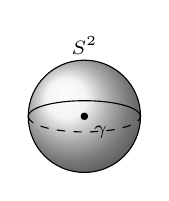
\begin{tikzpicture}[scale=0.62]
    \shade[ball color=black!6] (0,0) circle (1.15);
    \draw (0,0) circle (1.15);
    \draw[dashed] (-1.15,0) arc (180:360:1.15 and 0.32);
    \draw (-1.15,0) arc (180:0:1.15 and 0.32);
    \fill (0,0) circle (2.2pt) node[below right,font=\scriptsize]{$\gamma$};
    \node[font=\scriptsize] at (0,1.45) {$S^2$};
  \end{tikzpicture}
  \end{center}
  但 't Hooft 原来的定义对几何 Langlands 来说不够精确。
\end{frame}

\begin{frame}{Kapustin 的精确化}
  \srcp{44} Kapustin（2005）给了更精确的定义。他的讨论与 't Hooft 不同之处在于：
  他对奇点附近施加更精确的条件，而不只是指定情形的拓扑。
  \vspace{0.4em}

  \srcp{45} 想法是：要求场在 $\gamma$ 附近渐近于杨--米尔斯方程的一个指定的奇异解。
  对余维 $3$ 奇点的局部模型，可以取 $\RR^3$ 原点处的行为。对 $G=U(1)$，荷 $1$ 的
  “狄拉克单极子”解是一个曲率为
  \[
    F_0=\tfrac12\star\dd\frac{1}{|\vec x|}
  \]
  的联络 $A_0$。对任何 $G$（李代数为 $\mathfrak g$），取同态 $\rho:u(1)\to\mathfrak g$，
  并要求在 $\vec x=0$ 附近
  \[
    A\;\sim\;A_\rho:=\rho(A_0).
  \]
\end{frame}

\begin{frame}{型：一个余权}
  \srcp{46} 由于我们只关心 $A_\rho$ 在共轭意义下的类，可以把 $\rho$ 看成到极大环面
  $\mathfrak t$ 的同态：
  \[
    \rho:u(1)\to\mathfrak t ,
  \]
  再模去 Weyl 变换。于是“型”就是一个余权，模 Weyl 群：
  \[
    \{\text{'t Hooft 算子的型}\}\;\cong\;X_*(T)/W .
  \]
  \begin{beizhu}
  \textbf{批注}\quad 对比 Wilson 算子：它由表示 $R$ 标号，也就是由最高权
  $\rho_{\mathrm{el}}:T\to U(1)$ 标号，即 $X^*(T)/W$。
  电与磁，一个是权，一个是余权。这正是第 3 章那张表的物理版本。
  \end{beizhu}
\end{frame}

\begin{frame}{对照表}
  \begin{center}
  \renewcommand{\arraystretch}{1.45}
  \begin{tabular}{@{}lll@{}}
    \toprule
     & Wilson 算子 & 't Hooft 算子 \\
    \midrule
    定义 & 沿 $\gamma$ 的全纯的迹 & 沿 $\gamma$ 的指定奇点 \\
    标号 & $G$ 的表示 $R$ & 同态 $\rho_{\mathrm{mag}}:U(1)\to T$ \\
    群论数据 & 最高权 $\rho_{\mathrm{el}}:T\to U(1)$ & 余权 $\rho_{\mathrm{mag}}:U(1)\to T$ \\
    取值 & $X^*(T)$ & $X_*(T)$ \\
    对偶下 & $G$ 的 Wilson & $\gvee$ 的 't Hooft \\
    \bottomrule
  \end{tabular}
  \end{center}
\end{frame}

\begin{frame}{Montonen--Olive 下的交换}
  \srcp{48} 在规范群为 $G$ 与 $\gvee$ 的两个理论之间的 Montonen--Olive 对偶里，
  $G$ 的 Wilson 算子对应于 $\gvee$ 的 't Hooft 算子，反之亦然。依据是自然对应
  \[
    \rho:T\to U(1)
    \qquad\longleftrightarrow\qquad
    \rho^{\vee}:U(1)\to\Tvee
  \]
  以及 $G$ 与 $\gvee$ 有同一个 Weyl 群。
  \vspace{0.4em}

  这与 1977 年 GNO 的观察是同一件事；区别在于：改用线算子表述之后，
  不必再\textbf{调用希格斯机制}。
  \begin{beizhu}
  \textbf{批注}\quad 这正是 Witten 在 1977 年对 GNO 的不满所在：电与磁的匹配只在
  希格斯化之后才成立，而“根本性的陈述不应依赖希格斯化”。线算子的语言把它修好了。
  \end{beizhu}
\end{frame}

\begin{frame}{从粒子到算子：为什么要换语言}
  \begin{itemize}
    \item 粒子图像：磁荷 $\pi_1(G)$ 只在 $G$ 被破缺到 $T$ 之后才定义。
    \item 算子图像：'t Hooft 算子的型是一个余权，不依赖任何真空的选择。
    \item 好处：对偶成为关于\emph{算子}的陈述，可以在任意耦合下陈述与检验。
  \end{itemize}
  \vspace{0.5em}
  于是“GNO 的磁规范群 = Langlands 对偶群”从一个关于破缺相的事故，
  变成一个关于理论的\emph{结构性}事实。
\end{frame}

\partframe{八}{合流：$\RR\times C$ 上的 Bogomolny 方程}

\begin{frame}{与几何 Hecke 的关系}
  \srcp{49} 这一切与几何 Hecke 修改有什么关系？这里要考虑 Bogomolny 方程——
  它大致支配着四维超对称规范理论的\emph{时间无关}情形。
  \vspace{0.4em}

  在三维中，余维 $3$ 的奇点是一个孤立点：
  \begin{center}
  \begin{tikzpicture}[scale=1.0,>={Stealth[length=1.5mm]}]
    \draw (-1.5,-0.75) -- ++(3.0,0) -- ++(0.55,0.45) -- ++(-3.0,0) -- cycle;
    \draw[->] (0,0.35) -- (0,1.35) node[above,font=\scriptsize]{$\RR^3$};
    \fill[red] (0.9,0.15) circle (2.3pt);
    \node[font=\scriptsize,below right] at (0.95,0.1) {奇点};
  \end{tikzpicture}
  \end{center}
  所以要在 Dirac 型孤立奇点下解 Bogomolny 方程。这类问题最早由 Kronheimer（1986）
  与 Pauly（1990）研究。
\end{frame}

\begin{frame}{$\RR^3=\RR\times\RR^2$ 的两种读法}
  \srcp{50} Atiyah 与 Hitchin 在描述“谱曲线”时，把 $\RR^3$ 分解为 $\RR\times\RR^2$，
  看成 $\RR$ 的\emph{两参数}族。
  \vspace{0.4em}

  这里我们反过来：把 $\RR^3$ 看成 $\RR^2$ 的\emph{一参数}族。而且可以把 $\RR^2$
  换成任意 Riemann 面 $C$。所以我们研究 $\RR\times C$ 上的 Bogomolny 方程，
  把它看成 $C$ 的一参数族，用实变量 $y$ 参数化 $\RR$：
  \begin{center}
  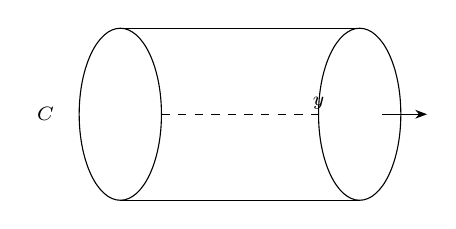
\begin{tikzpicture}[scale=0.95,>={Stealth[length=1.5mm]}]
    \draw (0,0) ellipse (0.55 and 1.15);
    \draw (3.2,0) ellipse (0.55 and 1.15);
    \draw (0,1.15) -- (3.2,1.15);
    \draw (0,-1.15) -- (3.2,-1.15);
    \draw[dashed] (0.55,0) -- (2.65,0);
    \node[font=\scriptsize] at (-1.0,0) {$C$};
    \node[font=\scriptsize] at (2.65,0.15) {$y$};
    \draw[->] (3.5,0) -- (4.1,0);
  \end{tikzpicture}
  \end{center}
  轴向是 $\RR$，每个横截面都是同一条 Riemann 面 $C$。
\end{frame}

\begin{frame}{Atiyah--Bott：全纯结构与 $y$ 无关}
  \srcp{51} 如 Atiyah 与 Bott 所解释的，$G$-丛 $E\to C$ 上的任何联络 $A$ 都决定一个
  全纯 $G_\CC$-丛 $E_\CC$：只需取 $A$ 的 $(0,1)$ 部分，用它来定义 $E$ 的复化上的全纯结构。
  \vspace{0.3em}

  因此 $C\times\RR$ 上的任何规范场 $A$ 都决定一族全纯丛 $E_y\to C$，$y\in\RR$。
  如果 $A$ 满足 Bogomolny 方程
  \[
    F=\star\dd_A\phi ,
  \]
  那么 $E_y$ 作为 $C$ 上的全纯丛，就\textbf{典范地}与 $y$ 无关。这是因为 Bogomolny
  方程的三个实分量中有两个可以写成
  \[
    0=\Bigl[\frac{D}{Dy}+i\phi,\;\frac{D}{D\bar z}\Bigr].
  \]
  第三个方程可以看成一个矩映射条件，类似 Atiyah 与 Bott 在讨论二维杨--米尔斯时所说的。
\end{frame}

\begin{frame}{跨过 $y_0$：一次 Hecke 修改}
  \srcp{52} 现在假设在某个点 $p\times y_0\in C\times\RR$ 处有一个 't Hooft/狄拉克奇点：
  \begin{center}
  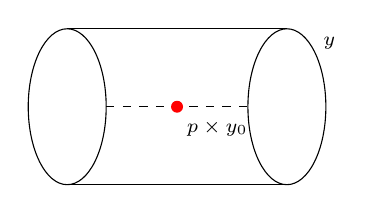
\begin{tikzpicture}[scale=0.9]
    \draw (0,0) ellipse (0.55 and 1.1);
    \draw (3.1,0) ellipse (0.55 and 1.1);
    \draw (0,1.1) -- (3.1,1.1);
    \draw (0,-1.1) -- (3.1,-1.1);
    \draw[dashed] (0.55,0) -- (2.55,0);
    \fill[red] (1.55,0) circle (2.4pt);
    \node[font=\scriptsize,below right] at (1.55,-0.05) {$p\times y_0$};
    \node[font=\scriptsize] at (3.7,0.9) {$y$};
  \end{tikzpicture}
  \end{center}
  那么 $E_y$ 除了 $y=y_0$ 外仍然典范地不依赖 $y$。即使跨过 $y=y_0$，只要把 $E_y$
  限制到 $C\setminus p$ 上，它仍然典范地不依赖 $y$。
  \vspace{0.3em}

  换句话说，在 $y=y_0$ 处发生的事情是：从 $E_y$ 在点 $p$ 作一次 \textbf{Hecke 修改}。
\end{frame}

\begin{frame}{型由奇点决定，对偶给出表示}
  Hecke 修改的“型”由那个特定的 't Hooft/狄拉克奇点决定，而它联系着
  $\rho:U(1)\to T$。
  \vspace{0.4em}

  电—磁对偶把它联系到某个
  \[
    \rho^{\vee}:\Tvee\to U(1),
  \]
  从而联系到对偶群的表示。几何 Hecke 修改与对偶群表示之间的这个关系，
  正是几何 Langlands 对应所断言的那个关系。
  \vspace{0.4em}
  \begin{beizhu}
  \textbf{批注}\quad 现在把三件事对齐：'t Hooft 奇点的型 $=$ 余权 $=$ Hecke 修改的型
  $=$ 对偶群的表示。物理的电磁对偶，恰好把最后一个等号的两端连了起来。
  \end{beizhu}
\end{frame}

\begin{frame}{两个模空间重合}
  \srcp{53} Bogomolny 方程解的模空间，与代数几何里定义的 Hecke 修改的模空间是重合的。
  这一点可以从“第三个”Bogomolny 方程的“矩映射”解释得出。
  \vspace{0.6em}

  \begin{center}
  \begin{tikzpicture}[>={Stealth[length=2mm]},node distance=1.5cm]
    \node[draw,rounded corners,inner sep=7pt,align=center] (a)
      {Bogomolny 解\\（模规范变换）};
    \node[draw,rounded corners,inner sep=7pt,align=center,right=2.6cm of a] (b)
      {Hecke 修改\\（代数几何）};
    \node[font=\scriptsize,below=0.55cm of a] (x) {矩映射条件};
    \node[font=\scriptsize,below=0.55cm of b] (y) {稳定条件};
    \draw[<->,thick] (a) -- node[above,font=\scriptsize]{$\cong$} (b);
  \end{tikzpicture}
  \end{center}
\end{frame}

\begin{frame}{收束}
  \srcp{54} 简而言之，我解释了规范理论对几何 Langlands 对应的解释里的某些主要想法。
  \begin{itemize}
    \item 我试着描述了这个故事如何从 1970 年代 Goddard、Nuyts、Olive 的工作开始，
      以及随后 Montonen 与 Olive 的工作；
    \item 我说了说这个故事如何与数学、物理中的其他发展并行展开；
    \item 我也解释了 Michael Atiyah 在这一过程中所起的影响。
  \end{itemize}
\end{frame}

\partframe{九}{补编：物理上怎么理解几何 Langlands}

\begin{frame}{一个自然的问题}
  Witten 的演讲到上一帧就结束了。但它留下一个没有正面回答的问题：
  \vspace{0.5em}
  \begin{center}
  \large 几何 Langlands 对应为什么应该是真的？
  \end{center}
  \vspace{0.5em}
  这不是“有没有证据”的问题，而是“它是不是某个更基本结构的影子”。
  2006 年，Kapustin 与 Witten 给出了一个答案；2008 年，Frenkel 与 Witten
  把它推进到内窥（endoscopy）。这一部分补上这条线。
  \begin{beizhu}
  \textbf{批注}\quad 以下不属于 Witten 2021 年演讲的原文，是译者根据
  Kapustin--Witten（2006）与 Frenkel--Witten（2008）补写的“下半场”。
  \end{beizhu}
\end{frame}

\begin{frame}{四维理论，二维约化}
  Kapustin--Witten 的出发点：取四维 $\cN=4$ 超杨--米尔斯理论，放在
  \[
    \RR\times\Sigma\times C
  \]
  上，其中 $C$ 是 Riemann 面，$\Sigma$ 是另一个曲面。先做拓扑扭化，再在 $\Sigma$ 上约化。
  \vspace{0.4em}

  结果是一个\textbf{二维 sigma 模型}，靶空间是 $C$ 上 $G$ 的 Hitchin 模空间：
  \[
    \mathcal M_H(G,C)=\Bigl\{(E,\phi)\;\Big|\;
    \bar\partial_A\phi=0,\; F_A+[\phi,\phi^*]=0\Bigr\}\Big/\!\sim .
  \]
  这里 $E\to C$ 是全纯 $G_\CC$-丛，$\phi\in H^0(C,\ad E\otimes K_C)$ 是 Higgs 场。
\end{frame}

\begin{frame}{Hitchin 模空间：三个复结构}
  $\mathcal M_H$ 是超 Kähler 流形：它有三个复结构 $I,J,K$，满足四元数关系。
  \begin{itemize}
    \item 在 $I$ 下：它是稳定 Higgs 丛的模空间；
    \item 在 $J$ 下：它是稳定平坦 $G_\CC$-丛的模空间（Corlette--Donaldson）；
    \item 复维数 $\dim_\CC\mathcal M_H=(2g-2)\dim G$。
  \end{itemize}
  \vspace{0.4em}
  它还是一个完全可积系统：Hitchin 纤维化
  \[
    \mathcal M_H\;\longrightarrow\;\bigoplus_{i=1}^{r}H^0(C,K_C^{\,d_i}),
  \]
  其纤维是 Prym 簇，谱曲线 $\det(\phi-\lambda)=0$ 控制着一切。
  \begin{beizhu}
  \textbf{批注}\quad 第 9 章里 Atiyah--Hitchin 用“谱曲线”描述单极子，用的正是同一个
  Hitchin 系统；只是那里 $C=\RR^2$ 被换成了复曲线，“谱曲线”才成为真正的代数曲线。
  \end{beizhu}
\end{frame}

\begin{frame}{S-对偶 = 镜像对称}
  $\cN=4$ 理论的 S-对偶：
  \[
    \tau\;\longmapsto\;-\frac{1}{n_g\tau},
    \qquad G\;\longmapsto\;\gvee ,
    \qquad \text{电}\;\longleftrightarrow\;\text{磁}.
  \]
  在二维 sigma 模型里，这个对偶变成了
  \[
    \mathcal M_H(G,C)\quad\longleftrightarrow\quad \mathcal M_H(\gvee,C)
  \]
  之间的\textbf{镜像对称}（在 Strominger--Yau--Zaslow 的意义上，纤维是环面）。
  \vspace{0.4em}

  这就是全部秘密：几何 Langlands 对应，是 Hitchin 模空间镜像对称的一个特例。
\end{frame}

\begin{frame}{算子与膜}
  扭化参数（记作 $\Psi$ 或 $t$）决定用 $\mathcal M_H$ 的哪一个复结构，从而决定
  得到的是 A-模型还是 B-模型。
  \vspace{0.4em}
  \begin{itemize}
    \item Wilson 算子与 't Hooft 算子分别实现 $\mathcal M_H$ 上的两类膜；
    \item S-对偶交换电与磁，也就交换这两类膜；
    \item 镜像对称把 A-膜与 B-膜互换。
  \end{itemize}
  \vspace{0.4em}
  于是“Wilson $\leftrightarrow$ 't Hooft”这个物理对偶，变成了
  “A-膜 $\leftrightarrow$ B-膜”这个几何陈述。
\end{frame}

\begin{frame}{特征层是膜，局部系统是点}
  几何 Langlands 的两侧，在 Hitchin 模空间上各是什么？
  \begin{itemize}
    \item \textbf{自守侧}：$\Bun_G$ 上的 Hecke 特征层 $\cF_\cE$。在 $\mathcal M_H$ 上，
      它实现为一个对 Hecke 算子本征的膜（eigenbrane）。
    \item \textbf{Galois 侧}：$C$ 上的 $\gvee$-局部系统 $\cE$。它对应
      $\mathcal M_H(\gvee,C)$ 里的一个点（更准确地说，一个 B-膜）。
  \end{itemize}
  \vspace{0.4em}
  镜像对称把点（B-膜）送到膜（A-膜）。这就是
  “特征层 $\leftrightarrow$ 局部系统”的物理内容。
  \begin{beizhu}
  \textbf{批注}\quad 这一帧是 2008 年 Frenkel--Witten 文章的核心图像之一。
  注意仍然有一环没合上：膜住在 $\mathcal M_H(G,C)$，而 D-模住在 $\Bun_G$；
  两者不是同一个空间，Kapustin--Witten 只在“非分歧”情形、并在某些极限下把两边对上。
  \end{beizhu}
\end{frame}

\begin{frame}{内窥：镜像对称预测数论}
  内窥（endoscopy）原本是 Langlands 函子性里的一类“函数转移”，涉及有相同对偶群的
  两个群。Frenkel 与 Witten（2008）指出：
  \begin{center}
  \begin{tabular}{@{}ll@{}}
    \toprule
    数论侧 & 几何/物理侧 \\
    \midrule
    内窥转移 & 两个 Hitchin 模空间之间的镜像对称 \\
    $L$-包 & 镜像对称下的膜对应 \\
    \bottomrule
  \end{tabular}
  \end{center}
  \vspace{0.4em}
  这不是“用物理解释已知的数学”，而是“用物理\emph{预测}了数学”：镜像对称给出了
  内窥转移的一个几何构造。这是这场演讲之后这条线最有说服力的进展之一。
\end{frame}

\begin{frame}{六维，以及 2024 年}
  \begin{itemize}
    \item Witten（2009）把整个构造提升到六维：六维 $(2,0)$ 理论在
      $\RR\times\Sigma\times C$ 上的边界条件，直接给出几何 Langlands 的两侧，
      不需要再额外“扭化”。
    \item 2024 年，Gaitsgory 与十余位合作者发表五篇论文，证明了非分歧情形下的
      几何 Langlands 猜想（对任意约化群）。
  \end{itemize}
  \vspace{0.4em}
  物理的“证明”仍是启发式的；但数学的证明已经落地，而这个证明用的中心对象
  （仿射 Grassmannian 上的几何 Satake 等价、$\Bun_G$ 上的 Hecke 特征层）正是
  演讲第 6 章介绍的那些。
\end{frame}

\begin{frame}{一张总表}
  \begin{center}
  \renewcommand{\arraystretch}{1.2}
  \begin{tabular}{@{}lll@{}}
    \toprule
    物理 & 群论 & 几何 \\
    \midrule
    电电荷 & $G$ 的表示 & $X^*(T)$ \\
    磁荷 & $\gvee$ 的表示 & $X_*(T)$ \\
    Wilson 算子 & 最高权 & $X^*(T)/W$ \\
    't Hooft 算子 & 余权 & $X_*(T)/W$ \\
    Hecke 修改 & $\gvee$ 的不可约表示 & 支配余权 \\
    S-对偶 & $G\leftrightarrow\gvee$ & $\mathcal M_H(G)\leftrightarrow\mathcal M_H(\gvee)$ \\
    \bottomrule
  \end{tabular}
  \end{center}
  \vspace{0.3em}
  \begin{center}\small
  这张表就是这场演讲的全部内容：四行物理，四行群论，四行几何，说的是同一件事。
  \end{center}
\end{frame}

\begin{frame}{时间线}
  \begin{center}
  \renewcommand{\arraystretch}{1.15}
  \small
  \begin{tabular}{@{}rl@{}}
    \toprule
    1977 & GNO：磁荷是权；Montonen--Olive：电—磁对偶 \\
    1978 & Witten--Olive：中心荷与 BPS 界 \\
    1979 & Osborn：只有 $\cN=4$ 满足判据 \\
    1990 & Beilinson--Drinfeld：几何 Langlands \\
    1994 & Sen 的束缚态；Seiberg--Witten 解 \\
    2005 & Kapustin：'t Hooft 算子的精确化 \\
    2006 & Kapustin--Witten：规范理论解释几何 Langlands \\
    2008 & Frenkel--Witten：几何内窥与镜像对称 \\
    2009 & Witten：六维 $(2,0)$ 构造 \\
    2021 & 本演讲 \\
    2024 & Gaitsgory 等：几何 Langlands 获证 \\
    \bottomrule
  \end{tabular}
  \end{center}
\end{frame}

\begin{frame}{术语速查}
  \begin{center}
  \renewcommand{\arraystretch}{1.15}
  \small
  \begin{tabular}{@{}lll@{}}
    \toprule
    英文 & 中文 & 一句话 \\
    \midrule
    dual group & 对偶群 & 交换特征标格与余特征标格 \\
    magnetic monopole & 单极子 & 磁荷的载体 \\
    't Hooft operator & 't Hooft 算子 & 沿曲线的指定奇点 \\
    Wilson operator & Wilson 算子 & 沿曲线的全纯的迹 \\
    Hecke modification & Hecke 修改 & 只在一点不同的两个丛 \\
    Hecke eigensheaf & Hecke 特征层 & 被 Hecke 算子本征化的层 \\
    geometric Satake & 几何 Satake 等价 & 反常层 $\leftrightarrow$ 对偶群表示 \\
    Hitchin moduli & Hitchin 模空间 & 超 Kähler，可积系统 \\
    BPS bound & BPS 界 & $M\ge|Z|$ \\
    \bottomrule
  \end{tabular}
  \end{center}
\end{frame}

\begin{frame}{延伸阅读}
  \footnotesize
  \begin{itemize}
    \item E. Witten, \emph{Duality, the Langlands Correspondence, and the Influence of
      Michael Atiyah}, INI, 2021（本演讲）。
    \item A. Kapustin, E. Witten, \emph{Electric-Magnetic Duality And The Geometric
      Langlands Program}, Commun. Number Theory Phys. 1 (2007) 1--236, hep-th/0604151.
    \item E. Frenkel, E. Witten, \emph{Geometric Endoscopy and Mirror Symmetry},
      Commun. Number Theory Phys. 2 (2008) 113--283, arXiv:0710.5939.
    \item E. Witten, \emph{Geometric Langlands From Six Dimensions}, arXiv:0905.2720.
    \item D. Gaitsgory et al., \emph{Proof of the geometric Langlands conjecture},
      five papers, 2024.
    \end{itemize}
  \vspace{0.2em}
  \begin{center}\scriptsize
  中译注本与资料卡：数译仓库 \texttt{papers/WIT-2021-ATIYAH-LANG}、
  \texttt{08\_source\_code/SY01-07}（几何内窥）、\texttt{datasets/kw06}。
  \end{center}
\end{frame}

\begin{frame}{}
  \vspace{2.2cm}
  \begin{center}
  {\Large\bfseries 谢谢}\\[0.8em]
  {\small 译文与批注：数译 · 超对称梦想家}\\[0.3em]
  {\small 底本：Edward Witten, INI, 2021-09-23}
  \end{center}
\end{frame}

\end{document}
